\chapter{Theoretical Background}
\label{ch:theory}

%=============================================================================
\section{Geostatistical framework: Ordinary Kriging}
\label{sec:theory-kriging}
%=============================================================================

\subsection{Spatial Random Fields}
\label{sec:random_fields}

Geostatistics treats a spatially distributed variable (such as daily
precipitation) as a realisation of a \textbf{spatial random field} (also
called a random function or stochastic process) $\{Z(\mathbf{s}) :
\mathbf{s} \in \mathcal{D}\}$, where $\mathbf{s} \in \mathbb{R}^2$ denotes a
spatial location and $\mathcal{D}$ is the study domain
\cite{matheron1963principles, cressie1993}.
Under this view, the observed precipitation values at weather stations are
treated as a single realisation of this random field, rather than as
deterministic quantities.

Hofstra et al.~\cite{hofstra2008comparison} describe kriging as a stochastic method in
which the interpolated value is a linear combination of nearby station
measurements, with weights chosen to minimise the mean squared prediction error
conditional on a model of spatial variability (the variogram).
Because these weights depend entirely on the distance-based covariance
structure, kriging implicitly relies on \textbf{spatial autocorrelation}: the
tendency of observations at nearby locations to be more similar than those at
distant locations.
Without such structure, the variogram would carry no information and there
would be no basis for predicting values at unobserved locations from nearby
measurements.
The following sections formalise this dependence structure through stationarity
assumptions and the variogram.


\subsection{Stationarity}
\label{sec:stationarity}

To make inference about a random field from a single realisation (the only
data available in practice), some regularity in the spatial structure
must be assumed.
The standard assumption is \textbf{stationarity}: the statistical properties
of the field do not depend on absolute location but only on the spatial
separation between points \cite{hofstra2008comparison, haylock2008european}.

\subsubsection{Second-Order Stationarity}

A random field is said to be \textit{second-order stationary} (or
\textit{weakly stationary}) if:

\begin{enumerate}
    \item The mean is constant: $E[Z(\mathbf{s})] = \mu$ for all
    $\mathbf{s} \in \mathcal{D}$.
    \item The covariance depends only on the separation vector $\mathbf{h}$:
    $\text{Cov}(Z(\mathbf{s}), Z(\mathbf{s} + \mathbf{h})) = C(\mathbf{h})$
    for all $\mathbf{s}$.
\end{enumerate}

\noindent Under this assumption, the covariance function $C(\mathbf{h})$
captures the full spatial dependence structure, and it can be estimated from
the data by treating all pairs of stations separated by lag $\mathbf{h}$ as
equivalent replicates \cite{cressie1993}.

\subsubsection{Intrinsic Stationarity}

Second-order stationarity requires a finite variance, which may not hold for
all natural processes.
A weaker condition, \textbf{intrinsic stationarity}, assumes only that the
variance of the increment $Z(\mathbf{s}+\mathbf{h}) - Z(\mathbf{s})$
depends on the lag~$\mathbf{h}$ alone and not on the location~$\mathbf{s}$:

\begin{equation}
    \text{Var}\bigl[Z(\mathbf{s} + \mathbf{h}) - Z(\mathbf{s})\bigr]
    = 2\gamma(\mathbf{h})
    \label{eq:intrinsic_stationarity}
\end{equation}

\noindent where $\gamma(\mathbf{h})$ is the \textbf{semi-variogram} (or simply
the variogram).
Intrinsic stationarity is sufficient for ordinary kriging and is the assumption
adopted throughout this work.
As Deutsch and Journel~\cite{deutsch1998gslib} note (Section~II.1.3, eq.~II.11), the
variogram definition requires only second-order stationarity of the random
function increments, a condition they call the \textit{``intrinsic hypothesis''}, which
is a weaker requirement than full second-order stationarity of the field
itself \cite{matheron1963principles, cressie1993}.

In the context of daily precipitation, raw observations violate stationarity in
two principal ways \cite{haylock2008european, hofstra2008comparison}.
The seasonal cycle introduces a large-scale trend, with the mean and
variance differing substantially between summer and winter months.
Orographic forcing also creates a spatial gradient in precipitation
climatology, with elevated regions receiving systematically more rainfall
than lowland areas \cite{haylock2008european}.
Both sources of non-stationarity must be removed before kriging can be
applied.


\subsection{The Variogram}
\label{sec:variogram}

\subsubsection{Definition and Estimation}

The semi-variogram $\gamma(\mathbf{h})$ defined in
Equation~\eqref{eq:intrinsic_stationarity} measures how the variance between
two observations grows with increasing separation $\mathbf{h}$.
In practice, the lag is treated as a scalar distance $h = \|\mathbf{h}\|$
under the isotropy assumption discussed in Section~\ref{sec:isotropy}.

The \textbf{empirical} (or \textit{experimental}) semi-variogram is estimated
from the data using the method-of-moments estimator
\cite{matheron1963principles}:

\begin{equation}
    \hat{\gamma}(h) =
    \frac{1}{2\,N(h)}
    \sum_{(i,j)\,:\,\|\mathbf{s}_i - \mathbf{s}_j\| \approx h}
    \bigl[Z(\mathbf{s}_i) - Z(\mathbf{s}_j)\bigr]^2
    \label{eq:empirical_variogram}
\end{equation}

\noindent where $N(h)$ is the number of station pairs whose distance falls
within the lag bin centred on $h$ \cite{cressie1993, haylock2008european}.
At least 30 pairs per lag bin are recommended to achieve statistical stability
\cite{cressie1993}.

\subsubsection{Key Parameters: Nugget, Sill, and Range}

A fitted variogram model is characterised by three parameters with clear
physical interpretations (Figure~\ref{fig:variogram_diagram}):

\begin{description}
    \item[Nugget ($c_0$)]
    The discontinuity at the origin: the variance between two measurements at
    the same location is theoretically zero, but empirical variograms typically
    show a positive intercept due to (i) measurement error in rain gauges and
    (ii) sub-grid spatial variability at scales smaller than the station
    spacing \cite{webster2007geostatistics}.
    For daily precipitation, the nugget reflects the fundamental
    unpredictability of highly localised convective cells.

    \item[Sill ($c_0 + c_1$)]
    The plateau reached by the variogram at large separations, equal to the
    overall variance of the transformed variable \cite{cressie1993}.
    The partial sill $c_1 = (c_0 + c_1) - c_0$ is the spatially structured
    component of the variance.
    For precipitation, the sill is larger for convective summer storms (high
    local variability) than for widespread stratiform winter events
    \cite{hofstra2008comparison}.

    \item[Range ($a$)]
    The separation distance at which the variogram reaches (or effectively
    reaches) the sill; beyond this distance, observations are spatially
    uncorrelated \cite{webster2007geostatistics}.
    Physically, the range reflects the spatial extent of the dominant weather
    system.
\end{description}

\noindent The \textbf{nugget-to-sill ratio} $c_0 / (c_0 + c_1)$ is a useful
diagnostic: values below 0.25 indicate strong spatial structure where kriging
adds substantial information beyond the sample mean, while values above 0.5
indicate that most variance is unstructured noise
\cite{webster2007geostatistics}.

\begin{figure}[ht]
    \centering
    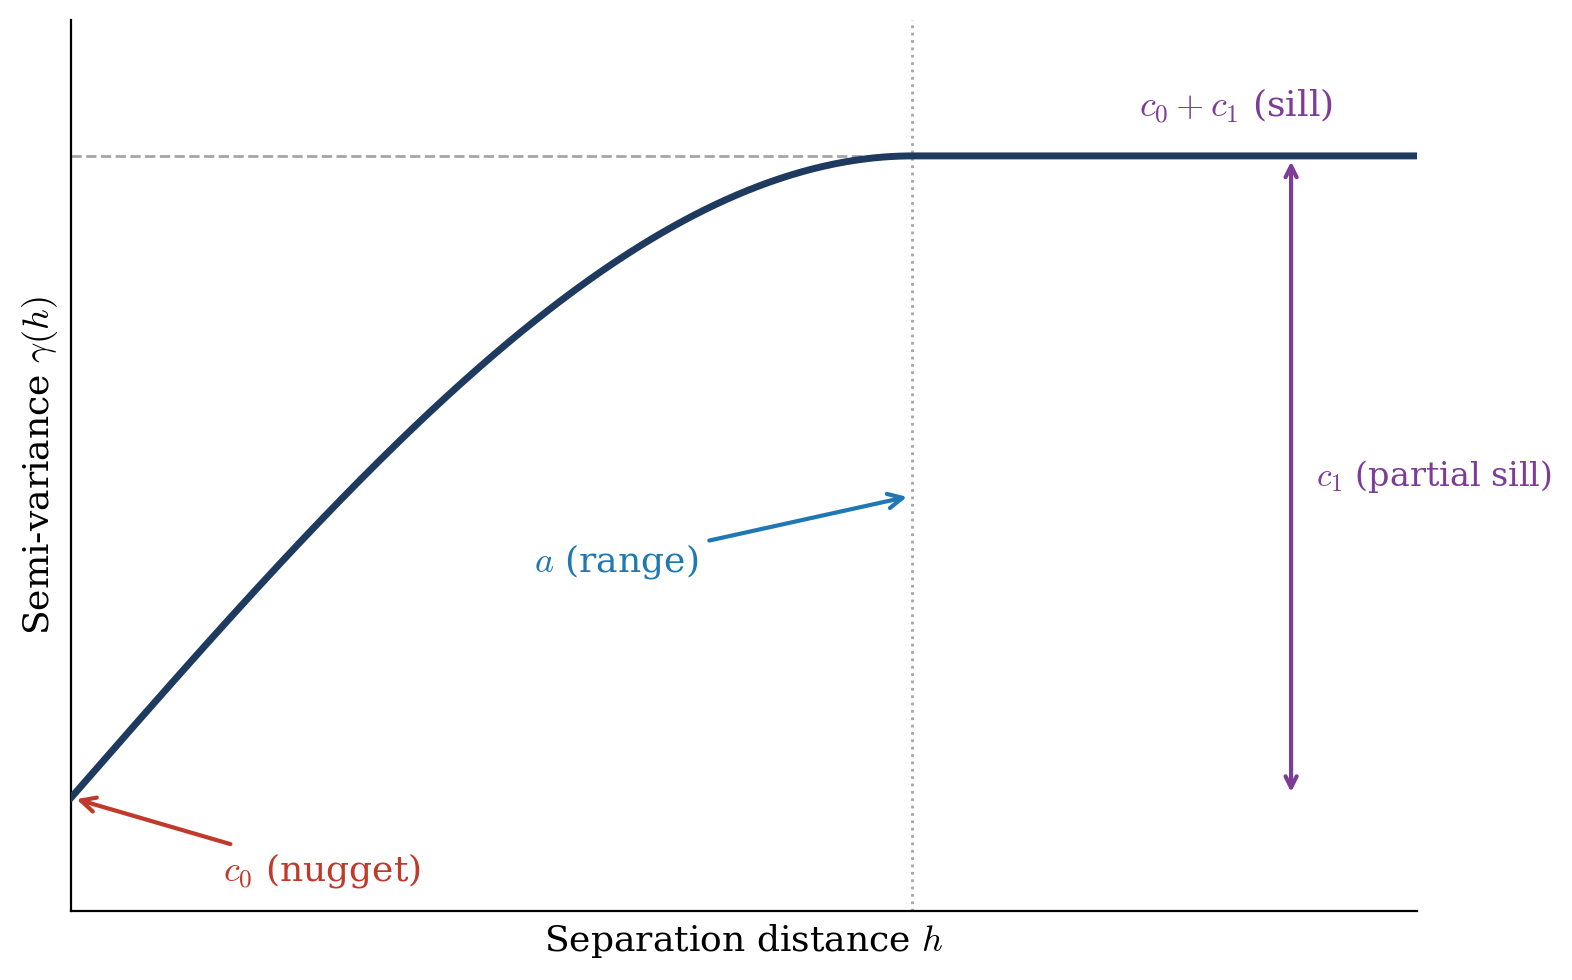
\includegraphics[width=0.85\textwidth]{images/02/variogram_diagram}
    \caption[Conceptual structure of a spherical variogram]{Conceptual structure of a spherical variogram, illustrating
    the three characteristic parameters: nugget $c_0$, partial sill $c_1$,
    sill $c_0 + c_1$, and range $a$; redrawn after Cressie~\cite{cressie1993}
    and Webster and Oliver~\cite{webster2007geostatistics}}
    \label{fig:variogram_diagram}
\end{figure}

\subsection{Variogram Models}
\label{sec:variogram_models}

A theoretical parametric model must be fitted to the empirical variogram before
it can be used in kriging, because the weights are computed from variogram
values at arbitrary distances not necessarily covered by the data.
The model must also be a \textit{valid} (conditionally negative
semi-definite) variogram, which guarantees that the kriging covariance
matrix is positive definite and the estimation variance is non-negative
\cite{cressie1993}.
All three models listed below satisfy this condition.

Three models are commonly used for precipitation
\cite[see][ch.~2--4]{cressie1993, webster2007geostatistics}:

\paragraph{Spherical model}

\begin{equation}
    \gamma_{\text{sph}}(h) =
    \begin{cases}
        c_0 + c_1 \!\left[\dfrac{3h}{2a} - \dfrac{1}{2}\!\left(\dfrac{h}{a}\right)^{\!3}\right]
        & h \le a \\[8pt]
        c_0 + c_1 & h > a
    \end{cases}
    \label{eq:spherical}
\end{equation}

The spherical model reaches the sill at a finite distance $a$ and is linear
near the origin, making it appropriate for variables that exhibit a sharp
decorrelation beyond a characteristic scale.
Haylock et al.~\cite{haylock2008european} recommend the spherical model for precipitation
\textit{occurrence} (indicator kriging).

\paragraph{Exponential model}

\begin{equation}
    \gamma_{\text{exp}}(h) = c_0 + c_1 \left[1 - \exp\!\left(-\frac{h}{a}\right)\right]
    \label{eq:exponential}
\end{equation}

The exponential model approaches the sill asymptotically; the effective range
(at which $\gamma$ reaches 95\% of the sill) is $3a$.
Unlike the spherical model, which reaches the sill at a finite distance,
the exponential model never fully decorrelates, making it appropriate for
precipitation \textit{amounts}, where spatial correlation
decays gradually over long distances \cite{haylock2008european}.

\paragraph{Gaussian model}

\begin{equation}
    \gamma_{\text{gau}}(h) = c_0 + c_1 \left[1 - \exp\!\left(-\frac{h^2}{a^2}\right)\right]
    \label{eq:gaussian}
\end{equation}

The Gaussian model is infinitely differentiable at the origin, implying
an extremely smooth spatial field.
While suitable for temperature fields, it is generally less appropriate for
precipitation because the parabolic behaviour near $h = 0$ tends to
underestimate short-range variability \cite{cressie1993}.

\subsubsection{Model Selection and Global Fitting}

In the E-OBS methodology, model parameters are estimated by the
\textbf{Marquardt method}~\cite{haylock2008european}, a weighted least squares
fit minimising the discrepancy between empirical and theoretical
variograms, with weights proportional to the number of station pairs per
lag bin:
\begin{equation}
  (c_0^*,\, c_1^*,\, a^*)
  = \argmin_{c_0,\, c_1,\, a}
    \sum_{k=1}^{K}
    N_k \!\left[\hat{\gamma}(h_k) - \gamma_{\theta}(h_k)\right]^{2},
  \label{eq:marquardt-variogram}
\end{equation}
where $N_k$ is the number of station pairs in bin~$k$, $\hat{\gamma}(h_k)$ is the
empirical semi-variance, and $\gamma_{\theta}(h_k)$ is the theoretical model.
Weighting by $N_k$ gives larger influence to well-populated bins, following the
E-OBS fitting procedure, which \textit{``gave more weight to those points in the
experimental variogram that were calculated from more station pairs''}
\cite[p.~5]{haylock2008european}.
Hofstra et al.~\cite{hofstra2008comparison} tested all three models and selected the best
fit using the chi-squared statistic.

A key practical finding is that a \textbf{global variogram}, fitted once by
pooling semi-variance estimates from many days, outperforms day-specific
variograms in cross-validation.
A variogram estimated from a single day's data (typically 100--200 pairs) is too
noisy: the standard error of the estimator is inversely proportional to
$\sqrt{N_k}$, where $N_k$ is the number of pairs at lag $k$.
Pooling across days provides a robust climatological
estimate of the spatial correlation structure
\cite{hofstra2008comparison, haylock2008european}.
Cross-validation experiments in both Haylock et al.~\cite{haylock2008european}
and Hofstra et al.~\cite{hofstra2008comparison} confirmed that a single global
variogram outperforms per-month fits: monthly subsets contain too few pairs for
a reliable estimate, and once precipitation is normalised by the monthly
climatology the residual correlation shape changes little between
seasons \cite{haylock2008european}.
This approach is adopted in the implementation described in
Chapter~\ref{ch:kriging}.


\subsection{Isotropy}
\label{sec:isotropy}

A variogram is called \textbf{isotropic} if it depends only on the distance
$h = \|\mathbf{h}\|$ and not on the direction of $\mathbf{h}$.
Anisotropy occurs when spatial correlation is stronger in one direction than
another (for example, along prevailing wind patterns or mountain ridges).

Hofstra et al.~\cite{hofstra2008comparison} tested for anisotropy in European daily
precipitation but found that computing directional variograms introduced more
uncertainty than it resolved, because fewer station pairs fall within each
directional bin.
They concluded that an omnidirectional (isotropic) variogram is more
appropriate for operational daily precipitation interpolation, and this choice
is followed throughout the present work.


\subsection{Ordinary Kriging as a Best Linear Unbiased Estimator}
\label{sec:kriging_blue}

\subsubsection{The Kriging Estimator}

Given observations $\{Z(\mathbf{s}_1), \ldots, Z(\mathbf{s}_n)\}$ at $n$
stations, the ordinary kriging estimator at an unobserved location $\mathbf{s}_0$
is defined as a \textbf{linear} combination of the observed values:

\begin{equation}
    \hat{Z}(\mathbf{s}_0) = \sum_{i=1}^{n} w_i \, Z(\mathbf{s}_i)
    \label{eq:kriging_estimator}
\end{equation}

\noindent where $w_i$ are weights to be determined
\cite{matheron1963principles, hofstra2008comparison}.

\subsubsection{Unbiasedness and the Weight Constraint}

For the estimator to be \textbf{unbiased}
($E[\hat{Z}(\mathbf{s}_0)] = E[Z(\mathbf{s}_0)] = \mu$), the weights must
sum to unity:

\begin{equation}
    \sum_{i=1}^{n} w_i = 1
    \label{eq:weight_constraint}
\end{equation}

\noindent This constraint ensures that kriging does not systematically
over- or under-predict the (unknown) spatial mean
\cite{cressie1993, hofstra2008comparison}.

\subsubsection{Optimality: Minimising the Estimation Variance}

The weights are chosen to minimise the \textbf{estimation variance}
(mean squared error):

\begin{equation}
    \sigma^2_{\text{OK}}(\mathbf{s}_0)
    = \text{Var}\!\left[\hat{Z}(\mathbf{s}_0) - Z(\mathbf{s}_0)\right]
    \label{eq:kriging_variance_def}
\end{equation}

\noindent subject to Constraint~\eqref{eq:weight_constraint}.
This is a constrained optimisation problem solved via a Lagrange multiplier
$\lambda$ \cite{cressie1993, webster2007geostatistics}.

\subsubsection{The Kriging System}

Taking partial derivatives with respect to each $w_i$ and setting them to
zero yields the \textbf{ordinary kriging system} in matrix form
\cite{cressie1993, webster2007geostatistics, deutsch1998gslib}:

\begin{equation}
    \begin{bmatrix}
        \mathbf{K} & \mathbf{1} \\
        \mathbf{1}^\top & 0
    \end{bmatrix}
    \begin{bmatrix}
        \mathbf{w} \\ \lambda
    \end{bmatrix}
    =
    \begin{bmatrix}
        \mathbf{k} \\ 1
    \end{bmatrix}
    \label{eq:kriging_system}
\end{equation}

\noindent where:
\begin{itemize}
    \item $K_{ij} = \gamma(\|\mathbf{s}_i - \mathbf{s}_j\|)$ is the
    $(n \times n)$ variogram matrix between all pairs of station locations,
    \item $k_i = \gamma(\|\mathbf{s}_i - \mathbf{s}_0\|)$ is the
    $(n \times 1)$ vector of variogram values between each station and
    the prediction point,
    \item $\mathbf{1}$ is an $n$-vector of ones enforcing
    Constraint~\eqref{eq:weight_constraint},
    \item $\lambda$ is the Lagrange multiplier.
\end{itemize}

Solving this $(n+1) \times (n+1)$ linear system yields the optimal weights
$\mathbf{w}^*$ and the Lagrange multiplier $\lambda^*$.
The associated kriging variance is:

\begin{equation}
    \sigma^2_{\text{OK}}(\mathbf{s}_0)
    = \sum_{i=1}^{n} w_i^* \, \gamma(\|\mathbf{s}_i - \mathbf{s}_0\|)
    + \lambda^*
    \label{eq:kriging_variance}
\end{equation}

\noindent This expression shows that the estimation uncertainty is large when
the prediction point is far from all stations (large $\gamma$ values) and
small when stations are nearby \cite{cressie1993}.

In summary, ordinary kriging is the BLUE because it is
\cite{matheron1963principles, cressie1993, webster2007geostatistics}:
\begin{itemize}
    \item \textbf{Linear} — the estimator is a weighted sum of observations
    (Equation~\eqref{eq:kriging_estimator}),
    \item \textbf{Unbiased} — the weight constraint ensures zero expected error
    (Equation~\eqref{eq:weight_constraint}),
    \item \textbf{Best} — the weights minimise the estimation variance among
    all linear unbiased estimators
    \cite{matheron1963principles, cressie1993}.
\end{itemize}

\noindent The BLUE property holds under the intrinsic stationarity assumption
and does not require a Gaussian distribution for the data.
Under approximate Gaussianity, the kriging variance
$\sigma^2_{\text{OK}}$ additionally acquires a probabilistic interpretation
as a prediction interval.

\subsection{Two-stage decomposition for zero-inflated data}
\label{sec:kriging-indicator}

The first and most fundamental decision when applying kriging to precipitation
is to decompose the task into two independent questions
rather than apply a single kriging model to the mixed distribution
\cite{journel1983indicator, haylock2008european}:

\begin{equation}
  Z(\mathbf{s}_0) =
    \underbrace{I(\mathbf{s}_0)}_{\text{stage 1: rain or not?}}
    \times
    \underbrace{A(\mathbf{s}_0)}_{\text{stage 2: how much?}}
  \label{eq:two-stage}
\end{equation}

In \textbf{Stage~1}, each observation is converted to a binary variable:
$I(\mathbf{s}_i, t) = 1$ if precipitation exceeds a wet-day threshold $\tau$, and $I = 0$ otherwise.
Ordinary Kriging is applied to these indicators and produces at each grid point a
value $\hat{p}(\mathbf{s}_0)$ interpreted as the probability of observing a wet day
\cite{hofstra2008comparison}.
Because ordinary kriging does not constrain predictions to $[0,1]$, values
slightly outside this range can occur near the boundaries of the wet--dry transition;
in practice a decision threshold $p^{\star}$ classifies a cell as rainy if
$\hat{p}(\mathbf{s}_0) > p^{\star}$.

The indicator semi-variogram $\gamma_I(h)$ describes how quickly agreement
in wet-day occurrence decays with spatial lag.
Following the global-variogram principle, a single spherical model is fitted by
pooling empirical indicator semi-variance across all days in the study period,
excluding constant days (all-wet or all-dry) on which the indicator has zero
variance.
Haylock et al.~\cite{haylock2008european} found that a global variogram produces
better interpolation skill than day-specific fits because the larger sample
provides a more statistically robust estimate of the spatial correlation
structure.
The fitted parameters of the global indicator variogram are applied
identically to every day, ensuring stable predictions even on days with
few wet stations where a per-day fit would be unreliable.

Ordinary Kriging (Section~\ref{sec:kriging_blue}) is applied to the binary
indicators, yielding the weighted estimate
$\hat{p}(\mathbf{s}_0, t) = \sum_{i=1}^{n} w_i\, I(\mathbf{s}_i, t)$
with weights from the kriging system~\eqref{eq:kriging_system}.
Because the input values are binary, this estimate is interpreted as the
wet-day probability at the target cell. The final first-stage decision is therefore
\begin{equation}
  \widehat{I}(\mathbf{s}_0, t)
  =
  \mathbf{1}\!\left[\hat{p}(\mathbf{s}_0, t) > p^{\star}\right].
  \label{eq:indicator-decision}
\end{equation}
Stage~1 thus outputs a binary wet/dry mask rather than precipitation amount in
millimetres.

In \textbf{Stage~2}, kriging is applied only to the positive observations (at those
stations where rain was recorded) and only for those grid cells where Stage~1 predicted
rainfall. The zero-inflation problem is resolved: the remaining mathematics operates
exclusively on the continuous distribution of positive precipitation amounts.

This coupling between the two stages can be written explicitly as
\begin{equation}
  \hat{Z}(\mathbf{s}_0, t)
  =
  \widehat{I}(\mathbf{s}_0, t)\, \hat{A}(\mathbf{s}_0, t),
  \label{eq:two-stage-predictor}
\end{equation}
where $\hat{A}(\mathbf{s}_0, t)$ is the second-stage amount prediction obtained only from
wet stations. If Stage~1 classifies the cell as dry, the final prediction is set to zero.

A practical limitation of the two-stage approach is that the final uncertainty
estimate is typically based only on Stage~2 (amount kriging) and does not account for the
classification uncertainty from Stage~1. Both questions, ``is it raining?'' and ``how
much?'', carry their own uncertainty, and combining them remains a non-trivial problem
\cite{haylock2008european}.

\subsection{Climatological normalisation}
\label{sec:theory-quota}

Having split the task into two stages, non-stationarity of the mean remains.
Consider the following: 10~mm of rainfall in June in a mountain foothills region is an
unremarkable event, roughly one sixth of the typical monthly normal. The same 10~mm in
December in Prague is anomalously high, twice the average. Kriging has no knowledge of
this distinction: both observations enter the interpolation equation with the same value
of ``10''.

The solution proposed in the E-OBS methodology \cite{haylock2008european} is to
replace absolute precipitation values with a \textbf{dimensionless climatological ratio}
indicating what fraction of the climatological monthly normal fell on that day:

\begin{equation}
  Q(\mathbf{s}_i, t) = \frac{Z(\mathbf{s}_i, t)}{\bar{M}(\mathbf{s}_i,\; m(t))}
  \label{eq:quota}
\end{equation}

where $\bar{M}(\mathbf{s}_i, m)$ is the long-term climatological monthly precipitation
total at station $\mathbf{s}_i$ in month $m$. This quantity is called the
\emph{quota} in the original E-OBS paper \cite{haylock2008european};
this thesis adopts the term \emph{ratio}, which is more transparent to a
general reader, but the symbol $Q$ and the construction are preserved.
After this normalisation, the expected value of the ratio is approximately constant
across all stations in any month: non-stationarity of the mean is eliminated,
and the kriging stationarity assumption is satisfied.
This procedure is an instance of \textbf{Climatologically Aided Interpolation}
(CAI) \cite{willmott1995cai}; the multiplicative ratio replaces the additive
deviation used for temperature, since precipitation variance scales with
the mean.

\subsection{Precipitation transforms}
\label{sec:kriging-nst}

After detrending, the wet-day ratios $Q$ are positive and approximately stationary,
but their distribution remains right-skewed and heavy-tailed
\cite{hofstra2008comparison, cecinati2017}.
Under Gaussianity, Ordinary Kriging additionally becomes the Best Linear Unbiased
\emph{Predictor} (BLUP), and the kriging variance acquires a correct probabilistic
interpretation as a prediction interval \cite{cressie1993, deutsch1998gslib}.
This motivates testing transforms that push the ratios closer to normality
\cite{cecinati2017}.
Three candidates are considered, each mapping the ratio to a working
variable~$z$ in a different \emph{z-space}:

\begin{enumerate}
  \item \textbf{None (raw ratio).}  The simplest option: $z = Q$.  The
        variogram is fitted directly on ratio values; no back-transformation is
        needed beyond the final multiplication
        $\hat{Z} = \hat{Q}\,\bar{M}$.

  \item \textbf{Log transform.}  $z = \log(Q + \delta)$ with a small
        offset $\delta$ to prevent divergence for near-zero ratios.
        This is a parametric transform that implicitly assumes an
        approximately log-normal distribution.  Back-transformation is
        $\hat{Q} = \exp(\hat{z}) - \delta$.

  \item \textbf{Normal Score Transform (NST).}  A rank-based transform
        mapping $Q$ to $\mathcal{N}(0,1)$ via the empirical CDF
        \cite{cecinati2017, deutsch1998gslib}.
\end{enumerate}

Each transform produces a different z-space with its own scale, so the
variogram parameters (sill, range, nugget) are not comparable across
transforms, and each combination of transform and variogram model must
be evaluated independently.

%=============================================================================
\section{Gradient boosting for spatial regression}
\label{sec:theory-gbm}
%=============================================================================

\subsection{Gradient boosting}
\label{sec:theory-gbm-general}

Gradient boosting is a supervised learning framework that constructs a
predictor as an additive ensemble of weak learners, typically shallow
regression trees \cite{friedman2001greedy}. Starting from a constant initial
prediction, the model is updated stage-wise:
\begin{equation}
  F_t(\mathbf{x}) = F_{t-1}(\mathbf{x}) + \nu \, h_t(\mathbf{x}),
  \label{eq:gbm-additive}
\end{equation}
where each tree $h_t$ is fitted to the negative gradient of a differentiable
loss function evaluated at the current ensemble's predictions, and the
learning rate $\nu \in (0, 1]$ controls the contribution of each new tree.
This is equivalent to gradient descent in the function space of the
ensemble: the negative gradient is the pseudo-residual that points to where
the current model has the largest error.
Unlike kriging, which assumes a stationary spatial random field, gradient
boosting does not require a parametric distributional model and admits
auxiliary covariates (e.g.\ elevation, soil properties) directly as input
features.
The same two-stage decomposition for zero-inflated precipitation
introduced in Section~\ref{sec:kriging-indicator} carries over to gradient
boosting, with a binary classifier and a quantile regression model
replacing indicator and amount kriging respectively.

\subsection{LightGBM}
\label{sec:theory-lgbm}

LightGBM \cite{ke2017lightgbm} is a gradient boosting library designed for
training speed and low memory use. It introduces several optimisations over
the classical algorithm:
\begin{itemize}
  \item \textbf{Leaf-wise tree growth:} instead of growing all leaves at the
    same depth, the leaf with the largest expected loss reduction is split
    first, so the tree deepens where the loss is largest.
  \item \textbf{Histogram-based splitting:} continuous feature values are
    discretised into a fixed number of bins, reducing the cost of finding
    the best split from $\mathcal{O}(n)$ to $\mathcal{O}(\#\text{bins})$.
  \item \textbf{Gradient-Based One-Side Sampling (GOSS):} retains all
    instances with large gradients and randomly subsamples those with small
    gradients. The most informative samples are kept and training cost
    drops with the subsample size.
  \item \textbf{Exclusive Feature Bundling (EFB):} combines mutually exclusive
    sparse features into a single feature, lowering effective dimensionality.
  \item \textbf{Built-in regularisation:} L1/L2 weight penalties, row and
    feature subsampling, leaf-count constraints, and early stopping on a
    validation set jointly control overfitting.
\end{itemize}
These optimisations let LightGBM scale to spatial precipitation problems
in which the number of station-day records reaches tens of millions.

\subsection{Quantile regression for probabilistic prediction}
\label{sec:theory-gbm-quantile}

A standard regression model returns a point estimate $\hat{y}(\mathbf{x})$,
which is insufficient for evaluation under a proper scoring rule such as
CRPS (Section~\ref{sec:theory-metrics}): the latter requires a full
predictive distribution, not a single value.
Quantile regression \cite{koenker1978regression} extends regression by
estimating conditional quantiles directly. For a target quantile level
$\tau \in (0, 1)$, the \textbf{pinball loss} (or check function)
\begin{equation}
  \rho_\tau(y - \hat{y})
    = \begin{cases}
      \tau\,(y - \hat{y})        & \text{if } y \geq \hat{y}, \\
      (\tau - 1)\,(y - \hat{y})  & \text{if } y < \hat{y},
    \end{cases}
  \label{eq:pinball}
\end{equation}
penalises under- and over-predictions asymmetrically in proportion to
$\tau$ and $1 - \tau$.
The conditional $\tau$-quantile estimator is then defined as the predictor
that minimises the average pinball loss over the training set
\cite{koenker1978regression}:
\begin{equation}
  \hat{f}_\tau
    = \argmin_{f \in \mathcal{F}}\,
      \frac{1}{n}\sum_{i=1}^{n} \rho_\tau\!\bigl(y_i - f(\mathbf{x}_i)\bigr).
  \label{eq:quantile-estimator}
\end{equation}
LightGBM supports the pinball loss as a built-in objective, so a separate
model can be trained for each desired quantile level $\tau$.
Predicting on a discrete grid of quantile levels yields an approximation
of the conditional predictive distribution, which serves as the ensemble
required for CRPS evaluation.
A closely related application of this approach is the satellite--gauge
precipitation merging study of Tyralis et al.~\cite{tyralis2023lightgbm},
who showed that LightGBM with quantile regression provides skilful
probabilistic predictions of daily precipitation, particularly at extreme
upper quantiles relevant for flood forecasting.

%=============================================================================
\section{Bayesian Neural Fields}
\label{sec:theory-bayesnf}
%=============================================================================

Ordinary kriging models a single scalar field with a globally stationary
semivariogram fitted to one variable, so auxiliary information such as
elevation, soil type, or seasonal regime can only be injected indirectly
through transforms and detrending stages. Bayesian Neural Fields (BayesNF)
\cite{saad2024bnf} replace this picture with a single Bayesian neural
network that maps spatiotemporal coordinates and arbitrary covariates to
a full predictive distribution, and that learns the covariance structure
of the field from the data rather than committing to a fixed parametric
form in advance.

\subsection{Architecture}
\label{sec:theory-bayesnf-arch}

BayesNF is a coordinate-based neural network: each input is the raw
$(\mathbf{s}, t, \mathbf{x}(\mathbf{s},t))$ tuple of location, time, and
covariates, and the output parameterises a distribution over the
observable field value $Y(\mathbf{s}, t)$. Because the network is
universal, the same backbone serves any spatiotemporal target without
manual redesign of the covariance model. Following Saad et al.\
\cite{saad2024bnf}, the model is hierarchical: a latent field
$F(\mathbf{s},t)$ together with global parameters $\Theta_f, \Theta_y$
defines the prior, and observations follow
\begin{equation}
  Y(\mathbf{s},t) \mid F(\mathbf{s},t), \Theta_y
    \;\sim\; \mathrm{Dist}\!\bigl(g(F(\mathbf{s},t)), \Theta_y\bigr),
  \label{eq:bnf-observation-model}
\end{equation}
where $\mathrm{Dist}$ is a configurable observation family and $g$ links
the latent field to its parameter~\cite{saad2024bnf}.
Figure~\ref{fig:bayesnf-architecture} shows the overall layer stack and
the parameters of the latent field $\theta_f$ and observation
model~$\theta_y$; the remainder of this section describes each layer in
turn.

\begin{figure}[ht]
    \centering
    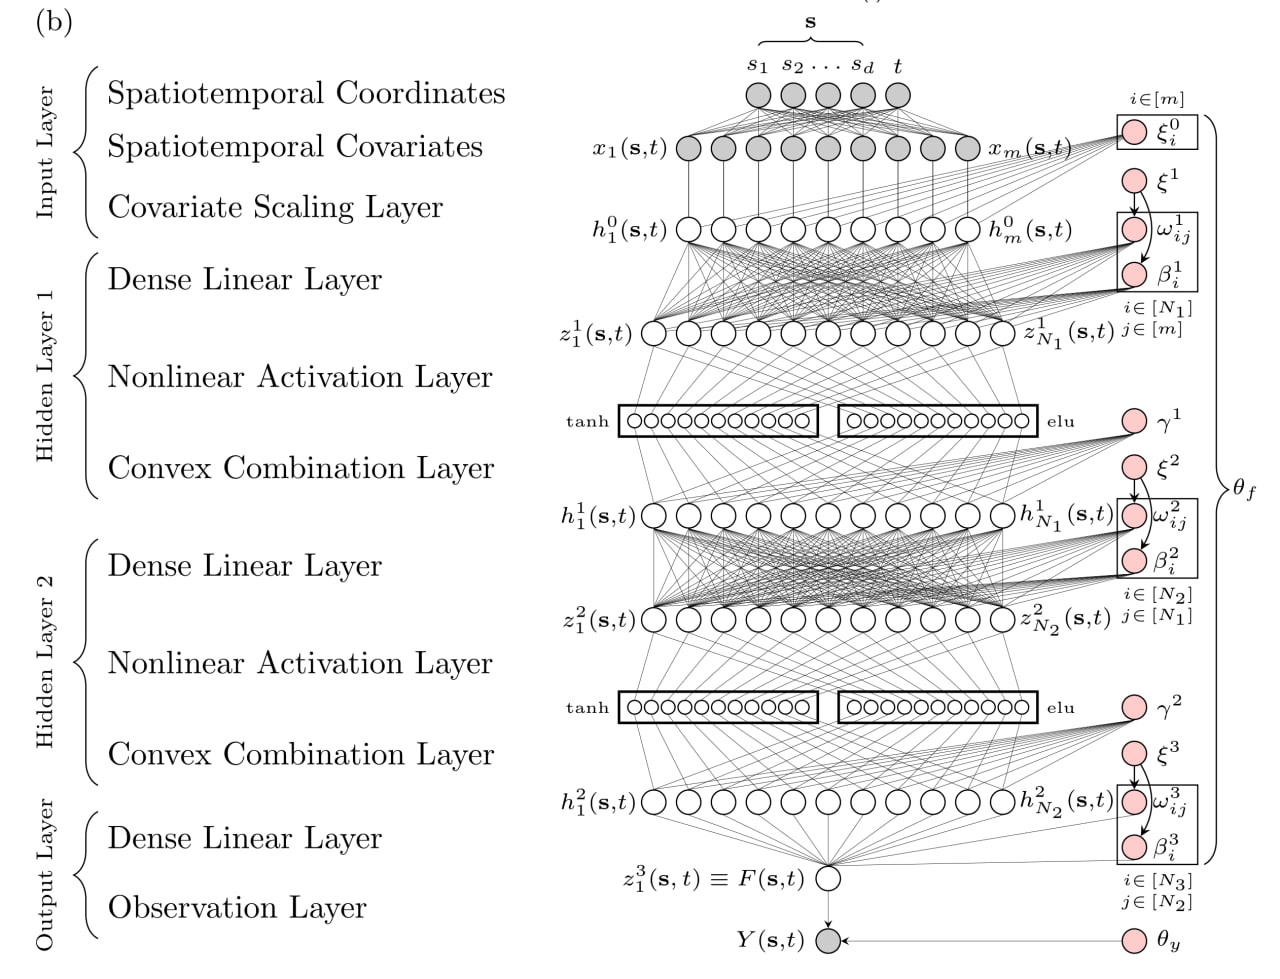
\includegraphics[width=0.95\textwidth]{images/06/bayesnf_architecture}
    \caption[BayesNF architecture]{Architecture of a Bayesian Neural
    Field with two hidden layers, after Saad et al.~\cite{saad2024bnf}}
    \label{fig:bayesnf-architecture}
\end{figure}

\subsubsection*{Covariate scaling layer}

This layer applies an element-wise rescaling
$\tilde{x}_i = e^{\xi_i}\,x_i$ with a learnable scale factor $e^{\xi_i}$
per covariate~\cite{saad2024bnf}. The appropriate scale is therefore
absorbed into the model parameters rather than requiring manual
standardisation of inputs, which otherwise heavily influences the
learning dynamics.

\subsubsection*{Fourier feature layer}

Plain multilayer perceptrons exhibit a \emph{spectral bias}: in the
neural tangent kernel limit they correspond to kernels with a rapid
frequency falloff, and therefore struggle to learn high-frequency
content from raw coordinates~\cite{tancik2020fourier}. Tancik et al.\
demonstrate that prepending a Fourier feature mapping transforms the
effective kernel into a stationary one with a tunable bandwidth, which
allows a multilayer perceptron to learn high-frequency functions in
low-dimensional problem domains~\cite{tancik2020fourier}. BayesNF adopts
this idea: each spatial axis $s_i$ is lifted into a bank of harmonics
\begin{equation}
  \phi_{s_i}(s_i) \;=\;
    \bigl\{\cos(2\pi\, 2^h\, s_i),\;\sin(2\pi\, 2^h\, s_i)\bigr\}_{h\in\mathcal{H}_{s_i}},
  \label{eq:bnf-spatial-fourier}
\end{equation}
and an analogous seasonal encoding is applied to the time axis with
period lengths chosen for the data's natural calendar
units~\cite{saad2024bnf}. This construction is theoretically justified
by the random Fourier feature framework of Rahimi and
Recht~\cite{rahimi2007rff}: Bochner's theorem characterises every
continuous shift-invariant positive-definite kernel on $\mathbb{R}^d$
as the Fourier transform of a non-negative measure, and the inner
product of two random Fourier feature vectors gives an unbiased Monte
Carlo estimate of that kernel. Combining Fourier features with a deep
neural prior therefore yields an expressive, data-driven covariance
structure rather than a pre-specified one. The empirical importance of
this layer is confirmed by an ablation study in Saad et al., which
reports substantial increases in RMSE, MAE, and MIS across most
benchmarks when the spatial Fourier features are
removed~\cite{saad2024bnf}.

\subsubsection*{Hidden layers with mixed activations}

The Fourier-encoded inputs are passed through $L+1 \geq 1$ dense hidden
layers. The non-linearity at each layer is a learnable softmax-weighted
convex combination of a small set of primitive activations, typically
$\{\tanh, \mathrm{relu}, \mathrm{elu}\}$~\cite{saad2024bnf}. This design
draws on the theory of expressive priors in Bayesian neural networks. In
the infinite-width limit, a Bayesian neural network converges to a
Gaussian process whose kernel is determined by the choice of activation
function: Pearce et al.\ show that swapping activation functions
effectively swaps the parametric form of the kernel, and that combining
several activations within an architecture induces a corresponding
combination of the underlying kernels~\cite{pearce2020expressive}.
BayesNF specialises this construction to a learnable softmax-weighted
convex combination, which Saad et al.\ motivate as a way to automate the
discovery of the covariance structure of the field, given that
activation functions correspond directly to the covariance of random
functions defined by Bayesian neural networks~\cite{saad2024bnf}.
Epistemic uncertainty is expressed by placing prior distributions over
all learnable parameters of the network, including the covariate scale
factors, the connection weights and biases, and the convex combination
coefficients.

\subsubsection*{Observation layer}

The hidden stack returns a real-valued latent field $F(\mathbf{s},t)$,
whereas the observable $Y(\mathbf{s},t)$ in this work is a non-negative
precipitation amount with a point mass at zero and a heavy right tail.
The \textbf{observation layer} maps $F(\mathbf{s},t)$ together with a
small set of global noise parameters $\Theta_y$ to a parametric
distribution $\mathrm{Dist}(\cdot;\,F(\mathbf{s},t),\Theta_y)$ on the
support of $Y$. The layer has two roles. First, it encodes the
\emph{aleatoric} uncertainty of the data-generating process: even if
$F$ were known exactly, $Y$ would remain random, and $\mathrm{Dist}$
specifies how. Second, it maps the unconstrained network output onto
the correct support, whether non-negative reals, non-negative integers,
or a zero-inflated mixture of the two, through a link function tied to
the choice of family. The choice of $\mathrm{Dist}$ therefore encodes
prior knowledge about the marginal distribution of the target and
dictates both the discretisation requirements on $Y$ and the form of
the predictive distribution at inference time.

The reference \texttt{google/bayesnf} implementation ships three
families~\cite{bayesnfRepo}:
\begin{description}
  \item[\texttt{NORMAL}] $Y(\mathbf{s},t) \sim
    \mathcal{N}\!\bigl(F(\mathbf{s},t),\,\sigma^{2}\bigr)$
    with a single learned noise scale~$\sigma$. Used for
    approximately Gaussian, real-valued targets.
  \item[\texttt{NB}] negative binomial with mean
    $\mu(\mathbf{s},t)=\mathrm{softplus}(F(\mathbf{s},t))$ and a learned
    dispersion shape~$\alpha$, so that
    $\mathrm{Var}[Y] = \mu + \alpha\,\mu^{2}$~\cite{bayesnfRepo}.
    Used for non-negative integer counts with overdispersion.
  \item[\texttt{ZINB}] zero-inflated negative binomial combining a
    Bernoulli mass at zero with probability $\pi_{0}$ and the
    negative binomial above with probability $1-\pi_{0}$, where $\pi_{0}$
    is a global learned parameter shared across all
    $(\mathbf{s},t)$~\cite{bayesnfRepo}.
\end{description}
\texttt{ZINB} matches daily precipitation: the marginal distribution
contains both a dry-day spike at zero and a heavy-tailed continuous
component. It is the family used in Chapter~\ref{ch:bayesnf}. Because
\texttt{NB} and \texttt{ZINB} are defined on $\mathbb{N}_{0}$, the
continuous precipitation amount must be discretised before training;
the discretisation and the inverse mapping used at prediction time are
described in Chapter~\ref{ch:bayesnf}.

\subsection{Inputs and hyperparameters}
\label{sec:theory-bayesnf-data}

Because the network absorbs the role of variogram model, transform,
neighbourhood index, and wet-dry decomposition, the data interface of
BayesNF is minimal: the required input is a long-table data frame in
which each row corresponds to one observation and stores its longitude,
latitude, time stamp, the target value $y$, and any number of static or
time-varying covariates~\cite{bayesnfRepo}. The remaining design choices
reduce to four hyperparameters: the harmonic sets $\mathcal{H}_{s_i}$ and
seasonal period set, which encode prior
expectations about spatial detail and temporal seasonality; the depth and
width of the dense backbone; the observation family $\mathrm{Dist}$
matched to the target distribution; and the posterior inference
algorithm, discussed next.

\subsection{Inference}
\label{sec:theory-bayesnf-inference}

\begin{sloppypar}
The posterior over network parameters is analytically
intractable~\cite{saad2024bnf}, so BayesNF relies on approximate inference.
Two scalable schemes are used: stochastic maximum-a-posteriori (MAP)
estimation, which returns a single parameter mode per random seed and is
fast but loses much of the posterior uncertainty; and mean-field
stochastic variational inference (VI), which fits a factorised
posterior and recovers wider predictive distributions at additional
computational cost.
\end{sloppypar}

\medskip\noindent
BayesNF is therefore the third candidate evaluated experimentally in
this thesis, alongside Ordinary Kriging (Chapter~\ref{ch:kriging}) and
gradient-boosted trees (Chapter~\ref{ch:gbm}).

%=============================================================================
\section{Evaluation metrics}
\label{sec:theory-metrics}
\label{sec:theory-crps}
%=============================================================================

All three interpolation methods in this thesis are evaluated using two metrics
applied consistently across Chapters~\ref{ch:kriging}--\ref{ch:comparison}.

\textbf{Mean Absolute Error (MAE)} measures point prediction accuracy as the
average absolute difference between predicted and observed precipitation
\cite{willmott2005mae}:
\begin{equation}
  \mathrm{MAE} = \frac{1}{n}\sum_{i=1}^{n}\bigl|\hat{Z}_i - Z_i\bigr|,
  \label{eq:mae}
\end{equation}
where $\hat{Z}_i$ and $Z_i$ are the predicted and observed values in
millimetres. MAE is expressed in the same physical units as precipitation and
is straightforward to interpret: a MAE of 1~mm means predictions are off by
1~mm on average. It evaluates only the point estimate, however, and says
nothing about the quality of the predicted uncertainty.

To assess the \textbf{full predictive distribution} of a probabilistic model,
the \textbf{Continuous Ranked Probability Score (CRPS)} is used
\cite{gneiting2007strictly}:
\begin{equation}
  \mathrm{CRPS}(F,\, y)
    = \int_{-\infty}^{\infty}
      \bigl(F(z) - \mathbf{1}\{z \ge y\}\bigr)^{2}\,\mathrm{d}z,
  \label{eq:crps}
\end{equation}
where $F$ is the predicted cumulative distribution function and $y$ is the
observation.  Intuitively, CRPS measures the integrated squared distance
between the forecast CDF and the ``perfect'' CDF, a unit step function at the
observed value.  A lower CRPS indicates a predictive distribution that is both
well-calibrated (centred on the truth) and sharp (concentrated, not
unnecessarily wide).

\begin{figure}[H]
    \centering
    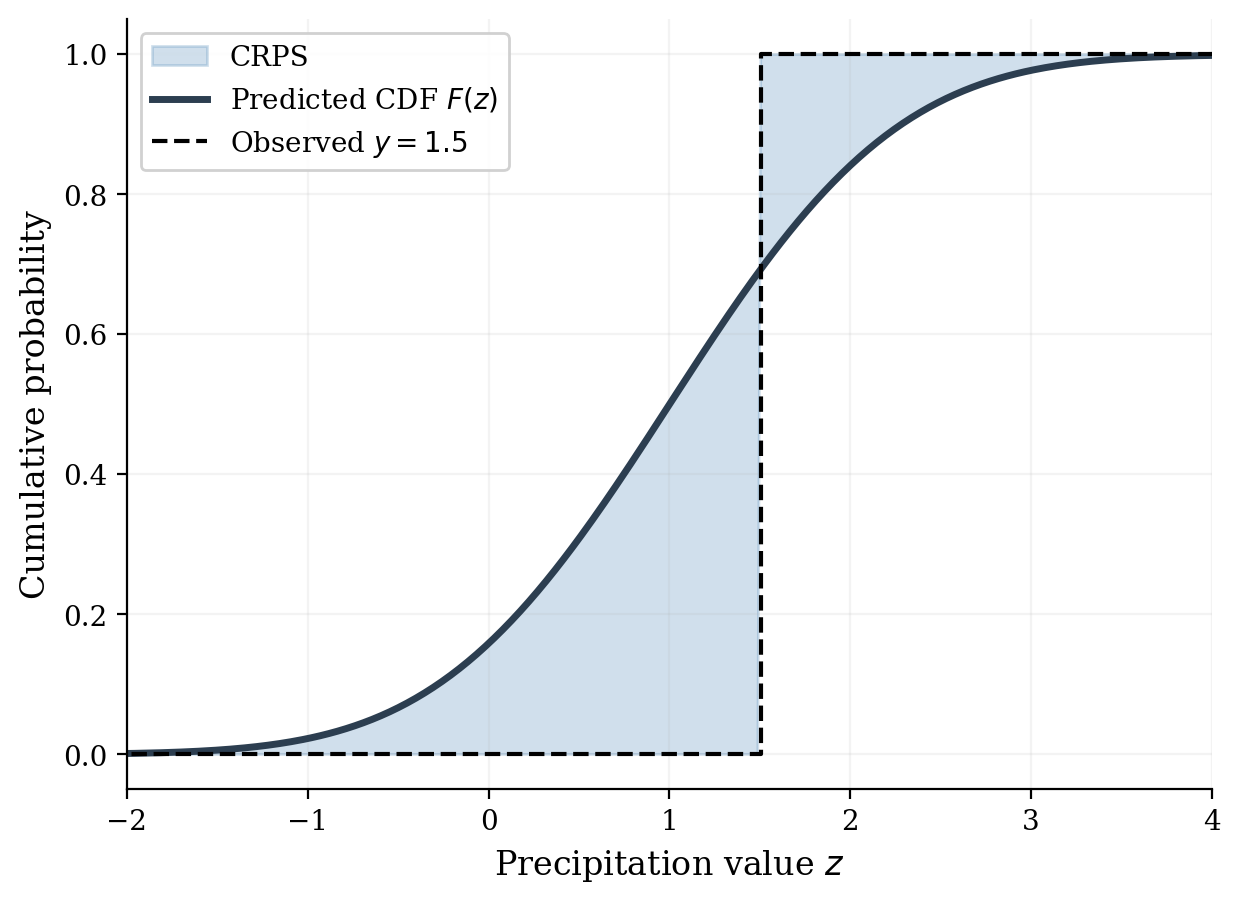
\includegraphics[width=0.85\textwidth]{images/02/crps_diagram}
    \caption[Geometric interpretation of CRPS]{Geometric interpretation of CRPS: the shaded area between the predicted CDF $F(z)$ and the step function at observed value~$y$; redrawn after Gneiting and Raftery~\cite{gneiting2007strictly}}
    \label{fig:crps-diagram}
\end{figure}

In practice the predictive distribution $F$ is rarely available in closed
form. Both the kriging and the gradient-boosting models in this work
represent $F$ by an ensemble of $M$ samples
$x_{1},\dots,x_{M}\sim F$ (for kriging, these are Monte-Carlo
back-transforms of Gaussian draws; see Equation~\eqref{eq:mc-backtrafo}). The
naive plug-in estimator that replaces $F$ by the empirical CDF of the
ensemble is biased downward at finite $M$ and only recovers the true CRPS in
the limit $M\!\to\!\infty$.  To obtain an unbiased estimate at any ensemble
size, the \textbf{fair CRPS estimator} of Ferro~\cite{ferro2014fair} is used:
\begin{equation}
  \widehat{\mathrm{CRPS}}_{\text{fair}}(x_{1:M},\,y)
    = \frac{1}{M}\sum_{m=1}^{M}\bigl|x_{m}-y\bigr|
    - \frac{1}{2\,M(M-1)}\sum_{m=1}^{M}\sum_{m'=1}^{M}\bigl|x_{m}-x_{m'}\bigr|.
  \label{eq:fair-crps}
\end{equation}
The first term measures the average distance of ensemble members to the
observation; the second is a finite-sample correction that subtracts the
ensemble's internal spread.  This estimator is unbiased for the population
CRPS under the standard assumption that ensemble members are exchangeable
draws from $F$, and it is the form actually computed in
Chapters~\ref{ch:kriging}--\ref{ch:comparison}.

CRPS is a \textbf{strictly proper scoring rule} for distributions with
finite first moment \cite{gneiting2007strictly}: its expectation is
minimised if and only if the predicted distribution equals the true
data-generating distribution.  This
means CRPS simultaneously penalises \emph{overconfidence} (intervals too narrow
that frequently miss the observation) and \emph{diffidence} (intervals too wide
that carry no useful information).  Unlike mean absolute error, CRPS therefore
provides a single number that rewards honest uncertainty quantification.

The root-mean-square error (RMSE), common in climatology, is \emph{not} used
in this work.  RMSE implicitly assumes Gaussian residuals, an assumption incompatible
with daily precipitation: the variable is non-negative, zero-inflated, and
heavy-tailed, so RMSE under-penalises rare extreme events and ignores the
large probability mass at zero \cite{hunt2025stop}.  CRPS, by contrast,
is a proper scoring rule that evaluates the full predictive distribution
without parametric assumptions, making it better suited to precipitation data.

